\documentclass[landscape,10pt]{article}
\usepackage[latin1]{inputenc}

\usepackage{ae}
\usepackage{amssymb}
\usepackage{url}
\usepackage{xspace}

\usepackage{tikz}
\usetikzlibrary{mindmap,trees}
\usetikzlibrary{shapes}

% set up externalization
\usetikzlibrary{external}
\tikzset{external/system call={latex \tikzexternalcheckshellescape -halt-on-error
-interaction=batchmode -jobname "\image" "\texsource";
dvips -o "\image".ps "\image".dvi;
ps2eps "\image.ps"}}
\tikzexternalize

%% https://www.bu.edu/math/files/2013/08/tikzpgfmanual.pdf

\begin{document}

\tikzstyle{root concept}+=[concept color=red!60]
%% \tikzstyle{level 1 concept}+=[set style={{every child}=[concept color=orange!50]}]
%% \tikzstyle{level 2 concept}+=[set style={{every child}=[concept color=blue!20]}]


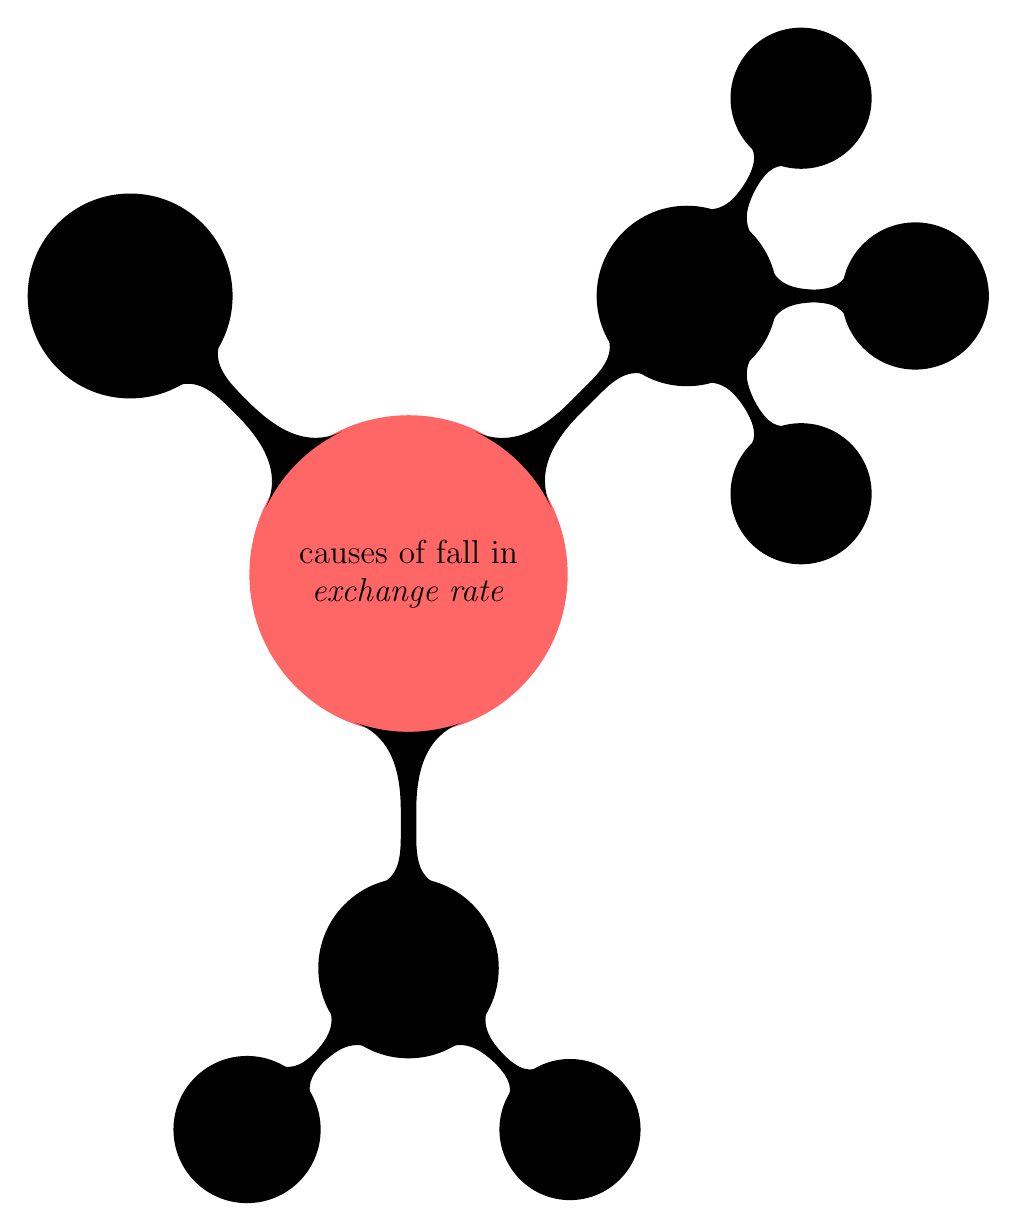
\begin{tikzpicture}[mindmap, level distance=30mm]
%%% 8-mark question %%%

      \node[concept, concept color=red!60] { causes of fall in\\ \emph{exchange rate} }
      %%
      child[grow=45] 
      {
        node[concept] { \textbf{definition}  }
        child[grow=60]  {node [concept] { \textbf{free float} } }
        child[grow=0]  {node [concept] { \textbf{fixed exchange rate} } }
        child[grow=-60]  {node [concept] { \textbf{managed float} } }
      }
      %% 
      child[grow=-90]
      {
        node[concept] { \textbf{floating exchange rate} }
        child[grow=-45]  {node [concept] { 
          \textbf{inflation} } 
          }
        child[grow=225]  {node [concept] { \textbf{lower interest rate} } }
      }
      child[grow=135] 
      {
        node[concept] { 
          \textbf{fixed exchange rate} \\ or \\ \textbf{managed float} 
          }
      }
      ;


\end{tikzpicture}



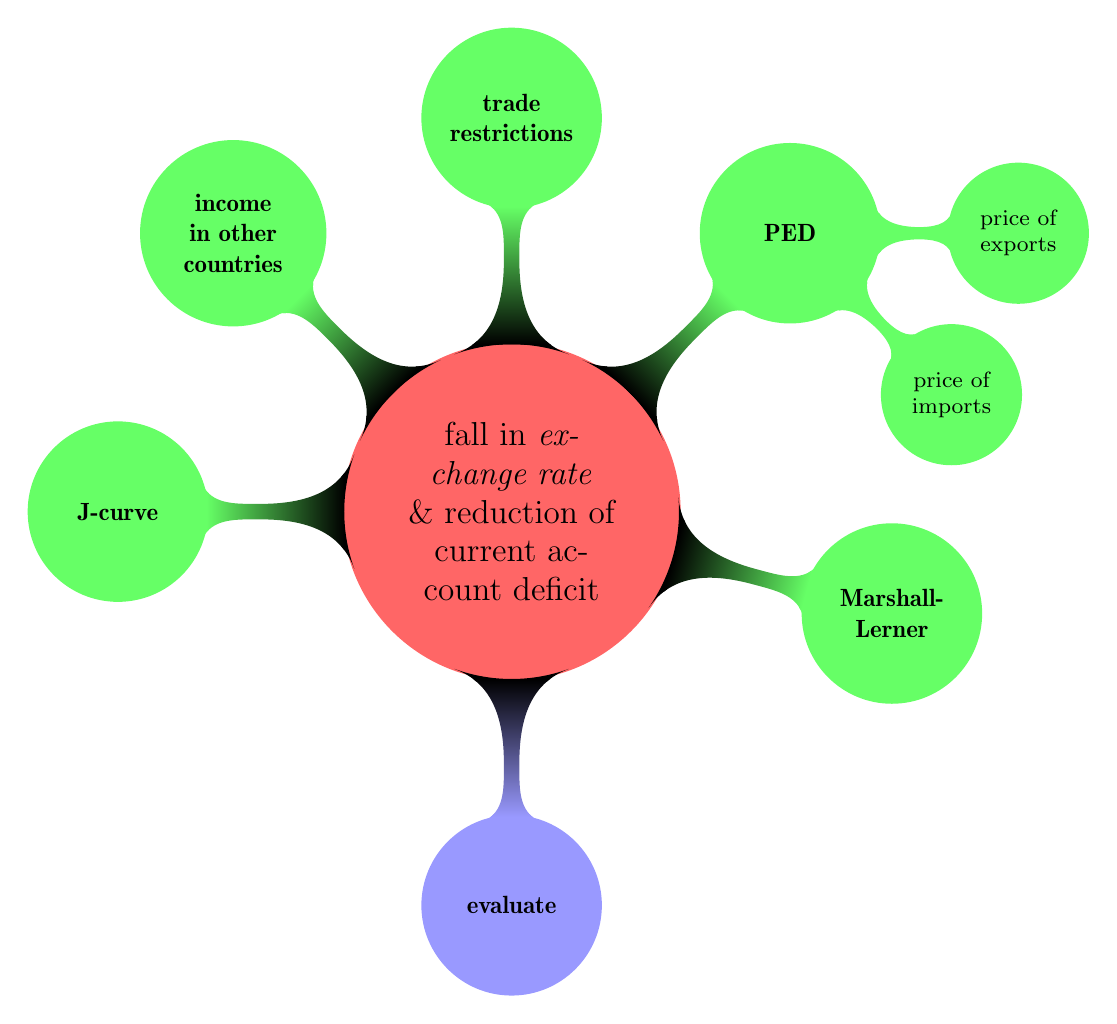
\begin{tikzpicture}[mindmap, level distance=30mm]
%%% 12-mark question %%%

      \node[concept, concept color=red!60] {fall in \emph{exchange rate}\\ \& reduction of \\ current account deficit }
      %% 
      child[grow=45, concept color=green!60]
      {
        node[concept, concept color=green!60] {\textbf{PED}}
        %
        child[grow=0, concept color=green!60]  {node [concept, concept color=green!60] { price of exports }}
        %
        child[grow=-45, concept color=green!60]  {node [concept] { price of imports }} 
      }
      %% 
      child[grow=-15, concept color=green!60]
      {
        node[concept, concept color=green!60] {\textbf{Marshall-Lerner}} 
      }
       %% 
      child[grow=-180, concept color=green!60]
      {
        node[concept, concept color=green!60] {\textbf{J-curve}} 
      }     
      %% 
      child[grow=135, concept color=green!60]
      {
        node[concept, concept color=green!60] {\textbf{income in other countries}} 
      }      
      %% 
      child[grow=90, concept color=green!60]
      {
        node[concept, concept color=green!60] {\textbf{trade restrictions}} 
      }      
      child[grow=-90, concept color=blue!40] 
      {
        node[concept, concept color=blue!40] {\textbf{evaluate} }
      }      
      ;


\end{tikzpicture}



\begin{tikzpicture}[mindmap, level distance=30mm]
%%% 8-mark question %%%

      \node[concept, concept color=red!60] { effect of \\ \emph{appreciation of currency} on\\ inflation rate }
      %%
      child[grow=45] 
      {
        node[concept] { \textbf{definition}  }
      }
      %% 
      child[grow=0]
      {
        node[concept] { \textbf{inflation calculation} }
      }
      %% 
      child[grow=-45]
      {
        node[concept] { \textbf{raw material \& input} }
      }
      %% 
      child[grow=-90]
      {
        node[concept] { \textbf{competitive-ness} }
      }      
      ;


\end{tikzpicture}



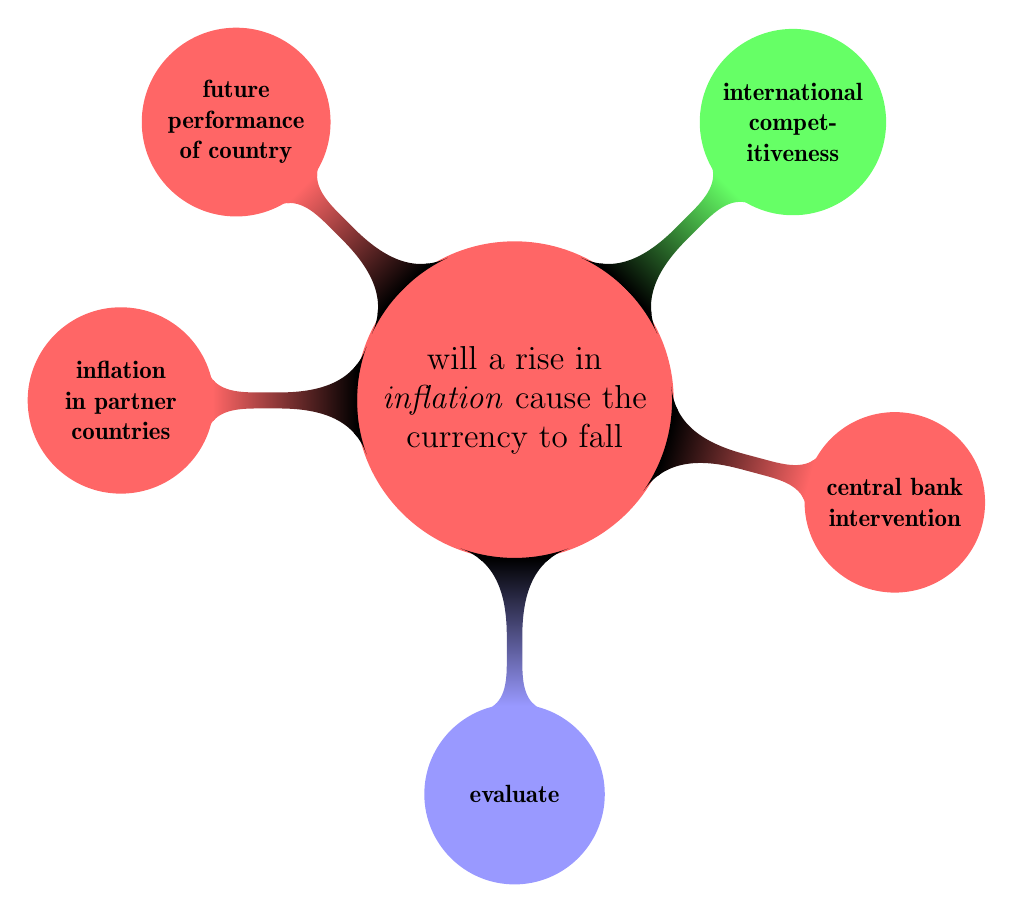
\begin{tikzpicture}[mindmap, level distance=30mm]
%%% 12-mark question %%%

      \node[concept, concept color=red!60] {will a rise in \emph{inflation} cause the currency to fall }
      %% 
      child[grow=45, concept color=green!60]
      {
        node[concept, concept color=green!60] {\textbf{international competitiveness}} 
      }
      %% 
      child[grow=-15, concept color=red!60]
      {
        node[concept, concept color=red!60] {\textbf{central bank intervention}} 
      }
       %% 
      child[grow=-180, concept color=red!60]
      {
        node[concept, concept color=red!60] {\textbf{inflation in partner countries}} 
      }     
      %% 
      child[grow=135, concept color=red!60]
      {
        node[concept, concept color=red!60] {\textbf{future performance of country}} 
      }      
      child[grow=-90, concept color=blue!40] 
      {
        node[concept, concept color=blue!40] {\textbf{evaluate} }
      }      
      ;


\end{tikzpicture}


\end{document}
